\subsubsection{The PoR Graph}

As a simplex ages, a graph of PoRs is produced (and it is a DAG).
Each vertex represents a block in some simplex-chain, and the outgoing edges point to reflected blocks.
An example section of a simulated PoR graph is shown in \autoref{fig:por-graph-example}.

\begin{figure}
\centering
\begin{comment}
    Generate the blocks and reflections data using this python script:

    ```python3
n_chains = 10
n_ticks = 32
overlap_each_tick = 3
prob_mine = overlap_each_tick / n_chains
print(f"expected blocks per chain: {n_ticks * prob_mine}")
chain_blocks = list(list(sum([(1 if random.random() < prob_mine else 0) for _ in range(attempts)]) for _ in range(n_ticks)) for _ in range(n_chains))
for chain in chain_blocks:
    print(f"{{{','.join(map(str,chain))}}},")

# generate code for the whole graph

print("\n\nTIKZ CODE FOR POR GRAPH BELOW\n\n")

def node_block(c, t):
    s = f"\\node ({nodename_of_block((c,t))}) [block] at ({t}*\\sx, {c}*\\sy) {{}};"
    return s

def node_invis(c, t):
    return f"\\node ({nodename_of_block((c,t))}) at ({t}*\\sx, {c}*\\sy) {{}};"

def nodename_of_block(ct: tuple[int, int]):
    c, t = ct
    return f"c{c}t{t}"

def edge_refl(ct_from, ct_to):
    s = f"\\draw [ar] ({nodename_of_block(ct_from)}) -- ({nodename_of_block(ct_to)});"
    return s

def edge_parent(ct_from, ct_to):
    s = f"\\draw [pAr] ({nodename_of_block(ct_from)}) -- ({nodename_of_block(ct_to)});"
    return s

def other_chains(local_c):
    return {c for c in range(n_chains) if c != local_c}

count_refls = 0

# loop through ticks and construct por graph segment
for t in range(n_ticks):
    for c in range(n_chains):
        blocks = chain_blocks[c]
        got_block = 1 == blocks[t]
        if got_block:
            print(node_block(c, t))
            # now to check for refls
            last_local_block = -1
            for prev_t in range(t - 1, -1, -1):
                if blocks[prev_t]:
                    last_local_block = prev_t
                    print(edge_parent((c,t), (c, prev_t)))
                    break
            # check to see if we're the first block
            if last_local_block < 0:
                print(node_invis(c, -1))
                print(edge_parent((c,t), (c, -1)))
            # we reflect any and all R blocks that were not in last local block's history
            for other_c in other_chains(c):
                for prev_t in range(t - 1, max(last_local_block - 1, -1), -1):
                    if chain_blocks[other_c][prev_t]:
                        print(edge_refl((c, t), (other_c, prev_t)))
                        count_refls += 1

# final arrows from future parents
for c in range(n_chains):
    blocks = chain_blocks[c]
    last_local_block = None
    for t in range(n_ticks - 1, -1, -1):
        if blocks[t]:
            last_local_block = t
            break
    else:
        raise Exception(f'no local blocks for chain {c}')
    print(node_invis(c, n_ticks))
    print(edge_parent((c, n_ticks), (c, last_local_block)))

print(f"\n\ncount_refls: {count_refls}")
    ```
\end{comment}

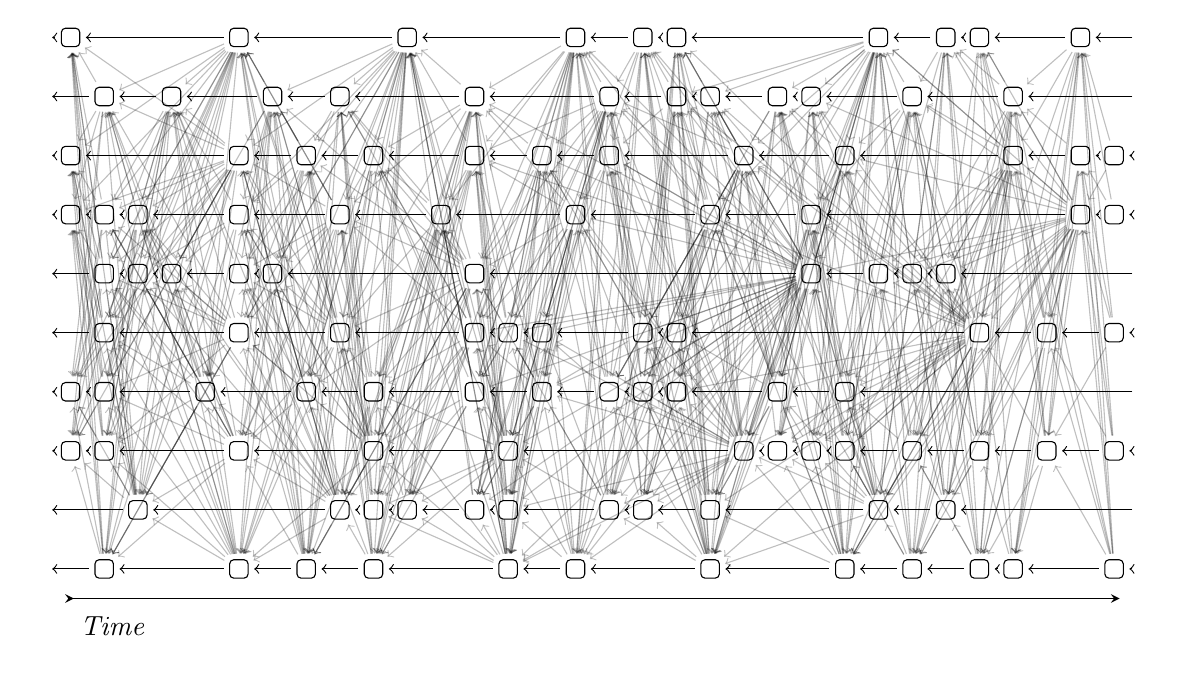
\begin{tikzpicture}[node distance=0.1cm]
    \tikzstyle{block} = [draw, rounded corners=1.5pt, fill=white]
    \tikzstyle{ar} = [->, -to, shorten >= 2pt, shorten <= 2pt, opacity=0.25]
    \tikzstyle{pAr} = [ar, opacity=1]
    \tikzstyle{arrowTime} = [stealth reversed-stealth, shorten >= -2pt, shorten <= -2pt]

    \def\scale{0.75cm}
    \edef\sx{2*0.285*\scale}
    \edef\sy{\scale}

    \def\timeArY{-0.5*\sy}
    \draw [arrowTime] (0, \timeArY) node () [anchor=west, yshift=-10pt] {\textit{Time}} -- (31*\sx, \timeArY);

    \node (c2t0) [block] at (0*\sx, 2*\sy) {};
    \node (c2t-1) at (-1*\sx, 2*\sy) {};
    \draw [pAr] (c2t0) -- (c2t-1);
    \node (c3t0) [block] at (0*\sx, 3*\sy) {};
    \node (c3t-1) at (-1*\sx, 3*\sy) {};
    \draw [pAr] (c3t0) -- (c3t-1);
    \node (c6t0) [block] at (0*\sx, 6*\sy) {};
    \node (c6t-1) at (-1*\sx, 6*\sy) {};
    \draw [pAr] (c6t0) -- (c6t-1);
    \node (c7t0) [block] at (0*\sx, 7*\sy) {};
    \node (c7t-1) at (-1*\sx, 7*\sy) {};
    \draw [pAr] (c7t0) -- (c7t-1);
    \node (c9t0) [block] at (0*\sx, 9*\sy) {};
    \node (c9t-1) at (-1*\sx, 9*\sy) {};
    \draw [pAr] (c9t0) -- (c9t-1);
    \node (c0t1) [block] at (1*\sx, 0*\sy) {};
    \node (c0t-1) at (-1*\sx, 0*\sy) {};
    \draw [pAr] (c0t1) -- (c0t-1);
    \draw [ar] (c0t1) -- (c2t0);
    \draw [ar] (c0t1) -- (c3t0);
    \draw [ar] (c0t1) -- (c6t0);
    \draw [ar] (c0t1) -- (c7t0);
    \draw [ar] (c0t1) -- (c9t0);
    \node (c2t1) [block] at (1*\sx, 2*\sy) {};
    \draw [pAr] (c2t1) -- (c2t0);
    \draw [ar] (c2t1) -- (c3t0);
    \draw [ar] (c2t1) -- (c6t0);
    \draw [ar] (c2t1) -- (c7t0);
    \draw [ar] (c2t1) -- (c9t0);
    \node (c3t1) [block] at (1*\sx, 3*\sy) {};
    \draw [pAr] (c3t1) -- (c3t0);
    \draw [ar] (c3t1) -- (c2t0);
    \draw [ar] (c3t1) -- (c6t0);
    \draw [ar] (c3t1) -- (c7t0);
    \draw [ar] (c3t1) -- (c9t0);
    \node (c4t1) [block] at (1*\sx, 4*\sy) {};
    \node (c4t-1) at (-1*\sx, 4*\sy) {};
    \draw [pAr] (c4t1) -- (c4t-1);
    \draw [ar] (c4t1) -- (c2t0);
    \draw [ar] (c4t1) -- (c3t0);
    \draw [ar] (c4t1) -- (c6t0);
    \draw [ar] (c4t1) -- (c7t0);
    \draw [ar] (c4t1) -- (c9t0);
    \node (c5t1) [block] at (1*\sx, 5*\sy) {};
    \node (c5t-1) at (-1*\sx, 5*\sy) {};
    \draw [pAr] (c5t1) -- (c5t-1);
    \draw [ar] (c5t1) -- (c2t0);
    \draw [ar] (c5t1) -- (c3t0);
    \draw [ar] (c5t1) -- (c6t0);
    \draw [ar] (c5t1) -- (c7t0);
    \draw [ar] (c5t1) -- (c9t0);
    \node (c6t1) [block] at (1*\sx, 6*\sy) {};
    \draw [pAr] (c6t1) -- (c6t0);
    \draw [ar] (c6t1) -- (c2t0);
    \draw [ar] (c6t1) -- (c3t0);
    \draw [ar] (c6t1) -- (c7t0);
    \draw [ar] (c6t1) -- (c9t0);
    \node (c8t1) [block] at (1*\sx, 8*\sy) {};
    \node (c8t-1) at (-1*\sx, 8*\sy) {};
    \draw [pAr] (c8t1) -- (c8t-1);
    \draw [ar] (c8t1) -- (c2t0);
    \draw [ar] (c8t1) -- (c3t0);
    \draw [ar] (c8t1) -- (c6t0);
    \draw [ar] (c8t1) -- (c7t0);
    \draw [ar] (c8t1) -- (c9t0);
    \node (c1t2) [block] at (2*\sx, 1*\sy) {};
    \node (c1t-1) at (-1*\sx, 1*\sy) {};
    \draw [pAr] (c1t2) -- (c1t-1);
    \draw [ar] (c1t2) -- (c0t1);
    \draw [ar] (c1t2) -- (c2t1);
    \draw [ar] (c1t2) -- (c2t0);
    \draw [ar] (c1t2) -- (c3t1);
    \draw [ar] (c1t2) -- (c3t0);
    \draw [ar] (c1t2) -- (c4t1);
    \draw [ar] (c1t2) -- (c5t1);
    \draw [ar] (c1t2) -- (c6t1);
    \draw [ar] (c1t2) -- (c6t0);
    \draw [ar] (c1t2) -- (c7t0);
    \draw [ar] (c1t2) -- (c8t1);
    \draw [ar] (c1t2) -- (c9t0);
    \node (c5t2) [block] at (2*\sx, 5*\sy) {};
    \draw [pAr] (c5t2) -- (c5t1);
    \draw [ar] (c5t2) -- (c0t1);
    \draw [ar] (c5t2) -- (c2t1);
    \draw [ar] (c5t2) -- (c3t1);
    \draw [ar] (c5t2) -- (c4t1);
    \draw [ar] (c5t2) -- (c6t1);
    \draw [ar] (c5t2) -- (c8t1);
    \node (c6t2) [block] at (2*\sx, 6*\sy) {};
    \draw [pAr] (c6t2) -- (c6t1);
    \draw [ar] (c6t2) -- (c0t1);
    \draw [ar] (c6t2) -- (c2t1);
    \draw [ar] (c6t2) -- (c3t1);
    \draw [ar] (c6t2) -- (c4t1);
    \draw [ar] (c6t2) -- (c5t1);
    \draw [ar] (c6t2) -- (c8t1);
    \node (c5t3) [block] at (3*\sx, 5*\sy) {};
    \draw [pAr] (c5t3) -- (c5t2);
    \draw [ar] (c5t3) -- (c1t2);
    \draw [ar] (c5t3) -- (c6t2);
    \node (c8t3) [block] at (3*\sx, 8*\sy) {};
    \draw [pAr] (c8t3) -- (c8t1);
    \draw [ar] (c8t3) -- (c0t1);
    \draw [ar] (c8t3) -- (c1t2);
    \draw [ar] (c8t3) -- (c2t1);
    \draw [ar] (c8t3) -- (c3t1);
    \draw [ar] (c8t3) -- (c4t1);
    \draw [ar] (c8t3) -- (c5t2);
    \draw [ar] (c8t3) -- (c5t1);
    \draw [ar] (c8t3) -- (c6t2);
    \draw [ar] (c8t3) -- (c6t1);
    \node (c3t4) [block] at (4*\sx, 3*\sy) {};
    \draw [pAr] (c3t4) -- (c3t1);
    \draw [ar] (c3t4) -- (c0t1);
    \draw [ar] (c3t4) -- (c1t2);
    \draw [ar] (c3t4) -- (c2t1);
    \draw [ar] (c3t4) -- (c4t1);
    \draw [ar] (c3t4) -- (c5t3);
    \draw [ar] (c3t4) -- (c5t2);
    \draw [ar] (c3t4) -- (c5t1);
    \draw [ar] (c3t4) -- (c6t2);
    \draw [ar] (c3t4) -- (c6t1);
    \draw [ar] (c3t4) -- (c8t3);
    \draw [ar] (c3t4) -- (c8t1);
    \node (c0t5) [block] at (5*\sx, 0*\sy) {};
    \draw [pAr] (c0t5) -- (c0t1);
    \draw [ar] (c0t5) -- (c1t2);
    \draw [ar] (c0t5) -- (c2t1);
    \draw [ar] (c0t5) -- (c3t4);
    \draw [ar] (c0t5) -- (c3t1);
    \draw [ar] (c0t5) -- (c4t1);
    \draw [ar] (c0t5) -- (c5t3);
    \draw [ar] (c0t5) -- (c5t2);
    \draw [ar] (c0t5) -- (c5t1);
    \draw [ar] (c0t5) -- (c6t2);
    \draw [ar] (c0t5) -- (c6t1);
    \draw [ar] (c0t5) -- (c8t3);
    \draw [ar] (c0t5) -- (c8t1);
    \node (c2t5) [block] at (5*\sx, 2*\sy) {};
    \draw [pAr] (c2t5) -- (c2t1);
    \draw [ar] (c2t5) -- (c0t1);
    \draw [ar] (c2t5) -- (c1t2);
    \draw [ar] (c2t5) -- (c3t4);
    \draw [ar] (c2t5) -- (c3t1);
    \draw [ar] (c2t5) -- (c4t1);
    \draw [ar] (c2t5) -- (c5t3);
    \draw [ar] (c2t5) -- (c5t2);
    \draw [ar] (c2t5) -- (c5t1);
    \draw [ar] (c2t5) -- (c6t2);
    \draw [ar] (c2t5) -- (c6t1);
    \draw [ar] (c2t5) -- (c8t3);
    \draw [ar] (c2t5) -- (c8t1);
    \node (c4t5) [block] at (5*\sx, 4*\sy) {};
    \draw [pAr] (c4t5) -- (c4t1);
    \draw [ar] (c4t5) -- (c0t1);
    \draw [ar] (c4t5) -- (c1t2);
    \draw [ar] (c4t5) -- (c2t1);
    \draw [ar] (c4t5) -- (c3t4);
    \draw [ar] (c4t5) -- (c3t1);
    \draw [ar] (c4t5) -- (c5t3);
    \draw [ar] (c4t5) -- (c5t2);
    \draw [ar] (c4t5) -- (c5t1);
    \draw [ar] (c4t5) -- (c6t2);
    \draw [ar] (c4t5) -- (c6t1);
    \draw [ar] (c4t5) -- (c8t3);
    \draw [ar] (c4t5) -- (c8t1);
    \node (c5t5) [block] at (5*\sx, 5*\sy) {};
    \draw [pAr] (c5t5) -- (c5t3);
    \draw [ar] (c5t5) -- (c3t4);
    \draw [ar] (c5t5) -- (c8t3);
    \node (c6t5) [block] at (5*\sx, 6*\sy) {};
    \draw [pAr] (c6t5) -- (c6t2);
    \draw [ar] (c6t5) -- (c1t2);
    \draw [ar] (c6t5) -- (c3t4);
    \draw [ar] (c6t5) -- (c5t3);
    \draw [ar] (c6t5) -- (c5t2);
    \draw [ar] (c6t5) -- (c8t3);
    \node (c7t5) [block] at (5*\sx, 7*\sy) {};
    \draw [pAr] (c7t5) -- (c7t0);
    \draw [ar] (c7t5) -- (c0t1);
    \draw [ar] (c7t5) -- (c1t2);
    \draw [ar] (c7t5) -- (c2t1);
    \draw [ar] (c7t5) -- (c2t0);
    \draw [ar] (c7t5) -- (c3t4);
    \draw [ar] (c7t5) -- (c3t1);
    \draw [ar] (c7t5) -- (c3t0);
    \draw [ar] (c7t5) -- (c4t1);
    \draw [ar] (c7t5) -- (c5t3);
    \draw [ar] (c7t5) -- (c5t2);
    \draw [ar] (c7t5) -- (c5t1);
    \draw [ar] (c7t5) -- (c6t2);
    \draw [ar] (c7t5) -- (c6t1);
    \draw [ar] (c7t5) -- (c6t0);
    \draw [ar] (c7t5) -- (c8t3);
    \draw [ar] (c7t5) -- (c8t1);
    \draw [ar] (c7t5) -- (c9t0);
    \node (c9t5) [block] at (5*\sx, 9*\sy) {};
    \draw [pAr] (c9t5) -- (c9t0);
    \draw [ar] (c9t5) -- (c0t1);
    \draw [ar] (c9t5) -- (c1t2);
    \draw [ar] (c9t5) -- (c2t1);
    \draw [ar] (c9t5) -- (c2t0);
    \draw [ar] (c9t5) -- (c3t4);
    \draw [ar] (c9t5) -- (c3t1);
    \draw [ar] (c9t5) -- (c3t0);
    \draw [ar] (c9t5) -- (c4t1);
    \draw [ar] (c9t5) -- (c5t3);
    \draw [ar] (c9t5) -- (c5t2);
    \draw [ar] (c9t5) -- (c5t1);
    \draw [ar] (c9t5) -- (c6t2);
    \draw [ar] (c9t5) -- (c6t1);
    \draw [ar] (c9t5) -- (c6t0);
    \draw [ar] (c9t5) -- (c7t0);
    \draw [ar] (c9t5) -- (c8t3);
    \draw [ar] (c9t5) -- (c8t1);
    \node (c5t6) [block] at (6*\sx, 5*\sy) {};
    \draw [pAr] (c5t6) -- (c5t5);
    \draw [ar] (c5t6) -- (c0t5);
    \draw [ar] (c5t6) -- (c2t5);
    \draw [ar] (c5t6) -- (c4t5);
    \draw [ar] (c5t6) -- (c6t5);
    \draw [ar] (c5t6) -- (c7t5);
    \draw [ar] (c5t6) -- (c9t5);
    \node (c8t6) [block] at (6*\sx, 8*\sy) {};
    \draw [pAr] (c8t6) -- (c8t3);
    \draw [ar] (c8t6) -- (c0t5);
    \draw [ar] (c8t6) -- (c2t5);
    \draw [ar] (c8t6) -- (c3t4);
    \draw [ar] (c8t6) -- (c4t5);
    \draw [ar] (c8t6) -- (c5t5);
    \draw [ar] (c8t6) -- (c5t3);
    \draw [ar] (c8t6) -- (c6t5);
    \draw [ar] (c8t6) -- (c7t5);
    \draw [ar] (c8t6) -- (c9t5);
    \node (c0t7) [block] at (7*\sx, 0*\sy) {};
    \draw [pAr] (c0t7) -- (c0t5);
    \draw [ar] (c0t7) -- (c2t5);
    \draw [ar] (c0t7) -- (c4t5);
    \draw [ar] (c0t7) -- (c5t6);
    \draw [ar] (c0t7) -- (c5t5);
    \draw [ar] (c0t7) -- (c6t5);
    \draw [ar] (c0t7) -- (c7t5);
    \draw [ar] (c0t7) -- (c8t6);
    \draw [ar] (c0t7) -- (c9t5);
    \node (c3t7) [block] at (7*\sx, 3*\sy) {};
    \draw [pAr] (c3t7) -- (c3t4);
    \draw [ar] (c3t7) -- (c0t5);
    \draw [ar] (c3t7) -- (c2t5);
    \draw [ar] (c3t7) -- (c4t5);
    \draw [ar] (c3t7) -- (c5t6);
    \draw [ar] (c3t7) -- (c5t5);
    \draw [ar] (c3t7) -- (c6t5);
    \draw [ar] (c3t7) -- (c7t5);
    \draw [ar] (c3t7) -- (c8t6);
    \draw [ar] (c3t7) -- (c9t5);
    \node (c7t7) [block] at (7*\sx, 7*\sy) {};
    \draw [pAr] (c7t7) -- (c7t5);
    \draw [ar] (c7t7) -- (c0t5);
    \draw [ar] (c7t7) -- (c2t5);
    \draw [ar] (c7t7) -- (c4t5);
    \draw [ar] (c7t7) -- (c5t6);
    \draw [ar] (c7t7) -- (c5t5);
    \draw [ar] (c7t7) -- (c6t5);
    \draw [ar] (c7t7) -- (c8t6);
    \draw [ar] (c7t7) -- (c9t5);
    \node (c1t8) [block] at (8*\sx, 1*\sy) {};
    \draw [pAr] (c1t8) -- (c1t2);
    \draw [ar] (c1t8) -- (c0t7);
    \draw [ar] (c1t8) -- (c0t5);
    \draw [ar] (c1t8) -- (c2t5);
    \draw [ar] (c1t8) -- (c3t7);
    \draw [ar] (c1t8) -- (c3t4);
    \draw [ar] (c1t8) -- (c4t5);
    \draw [ar] (c1t8) -- (c5t6);
    \draw [ar] (c1t8) -- (c5t5);
    \draw [ar] (c1t8) -- (c5t3);
    \draw [ar] (c1t8) -- (c5t2);
    \draw [ar] (c1t8) -- (c6t5);
    \draw [ar] (c1t8) -- (c6t2);
    \draw [ar] (c1t8) -- (c7t7);
    \draw [ar] (c1t8) -- (c7t5);
    \draw [ar] (c1t8) -- (c8t6);
    \draw [ar] (c1t8) -- (c8t3);
    \draw [ar] (c1t8) -- (c9t5);
    \node (c4t8) [block] at (8*\sx, 4*\sy) {};
    \draw [pAr] (c4t8) -- (c4t5);
    \draw [ar] (c4t8) -- (c0t7);
    \draw [ar] (c4t8) -- (c0t5);
    \draw [ar] (c4t8) -- (c2t5);
    \draw [ar] (c4t8) -- (c3t7);
    \draw [ar] (c4t8) -- (c5t6);
    \draw [ar] (c4t8) -- (c5t5);
    \draw [ar] (c4t8) -- (c6t5);
    \draw [ar] (c4t8) -- (c7t7);
    \draw [ar] (c4t8) -- (c7t5);
    \draw [ar] (c4t8) -- (c8t6);
    \draw [ar] (c4t8) -- (c9t5);
    \node (c6t8) [block] at (8*\sx, 6*\sy) {};
    \draw [pAr] (c6t8) -- (c6t5);
    \draw [ar] (c6t8) -- (c0t7);
    \draw [ar] (c6t8) -- (c0t5);
    \draw [ar] (c6t8) -- (c2t5);
    \draw [ar] (c6t8) -- (c3t7);
    \draw [ar] (c6t8) -- (c4t5);
    \draw [ar] (c6t8) -- (c5t6);
    \draw [ar] (c6t8) -- (c5t5);
    \draw [ar] (c6t8) -- (c7t7);
    \draw [ar] (c6t8) -- (c7t5);
    \draw [ar] (c6t8) -- (c8t6);
    \draw [ar] (c6t8) -- (c9t5);
    \node (c8t8) [block] at (8*\sx, 8*\sy) {};
    \draw [pAr] (c8t8) -- (c8t6);
    \draw [ar] (c8t8) -- (c0t7);
    \draw [ar] (c8t8) -- (c3t7);
    \draw [ar] (c8t8) -- (c5t6);
    \draw [ar] (c8t8) -- (c7t7);
    \node (c0t9) [block] at (9*\sx, 0*\sy) {};
    \draw [pAr] (c0t9) -- (c0t7);
    \draw [ar] (c0t9) -- (c1t8);
    \draw [ar] (c0t9) -- (c3t7);
    \draw [ar] (c0t9) -- (c4t8);
    \draw [ar] (c0t9) -- (c6t8);
    \draw [ar] (c0t9) -- (c7t7);
    \draw [ar] (c0t9) -- (c8t8);
    \node (c1t9) [block] at (9*\sx, 1*\sy) {};
    \draw [pAr] (c1t9) -- (c1t8);
    \draw [ar] (c1t9) -- (c4t8);
    \draw [ar] (c1t9) -- (c6t8);
    \draw [ar] (c1t9) -- (c8t8);
    \node (c2t9) [block] at (9*\sx, 2*\sy) {};
    \draw [pAr] (c2t9) -- (c2t5);
    \draw [ar] (c2t9) -- (c0t7);
    \draw [ar] (c2t9) -- (c0t5);
    \draw [ar] (c2t9) -- (c1t8);
    \draw [ar] (c2t9) -- (c3t7);
    \draw [ar] (c2t9) -- (c4t8);
    \draw [ar] (c2t9) -- (c4t5);
    \draw [ar] (c2t9) -- (c5t6);
    \draw [ar] (c2t9) -- (c5t5);
    \draw [ar] (c2t9) -- (c6t8);
    \draw [ar] (c2t9) -- (c6t5);
    \draw [ar] (c2t9) -- (c7t7);
    \draw [ar] (c2t9) -- (c7t5);
    \draw [ar] (c2t9) -- (c8t8);
    \draw [ar] (c2t9) -- (c8t6);
    \draw [ar] (c2t9) -- (c9t5);
    \node (c3t9) [block] at (9*\sx, 3*\sy) {};
    \draw [pAr] (c3t9) -- (c3t7);
    \draw [ar] (c3t9) -- (c0t7);
    \draw [ar] (c3t9) -- (c1t8);
    \draw [ar] (c3t9) -- (c4t8);
    \draw [ar] (c3t9) -- (c6t8);
    \draw [ar] (c3t9) -- (c7t7);
    \draw [ar] (c3t9) -- (c8t8);
    \node (c7t9) [block] at (9*\sx, 7*\sy) {};
    \draw [pAr] (c7t9) -- (c7t7);
    \draw [ar] (c7t9) -- (c0t7);
    \draw [ar] (c7t9) -- (c1t8);
    \draw [ar] (c7t9) -- (c3t7);
    \draw [ar] (c7t9) -- (c4t8);
    \draw [ar] (c7t9) -- (c6t8);
    \draw [ar] (c7t9) -- (c8t8);
    \node (c1t10) [block] at (10*\sx, 1*\sy) {};
    \draw [pAr] (c1t10) -- (c1t9);
    \draw [ar] (c1t10) -- (c0t9);
    \draw [ar] (c1t10) -- (c2t9);
    \draw [ar] (c1t10) -- (c3t9);
    \draw [ar] (c1t10) -- (c7t9);
    \node (c9t10) [block] at (10*\sx, 9*\sy) {};
    \draw [pAr] (c9t10) -- (c9t5);
    \draw [ar] (c9t10) -- (c0t9);
    \draw [ar] (c9t10) -- (c0t7);
    \draw [ar] (c9t10) -- (c0t5);
    \draw [ar] (c9t10) -- (c1t9);
    \draw [ar] (c9t10) -- (c1t8);
    \draw [ar] (c9t10) -- (c2t9);
    \draw [ar] (c9t10) -- (c2t5);
    \draw [ar] (c9t10) -- (c3t9);
    \draw [ar] (c9t10) -- (c3t7);
    \draw [ar] (c9t10) -- (c4t8);
    \draw [ar] (c9t10) -- (c4t5);
    \draw [ar] (c9t10) -- (c5t6);
    \draw [ar] (c9t10) -- (c5t5);
    \draw [ar] (c9t10) -- (c6t8);
    \draw [ar] (c9t10) -- (c6t5);
    \draw [ar] (c9t10) -- (c7t9);
    \draw [ar] (c9t10) -- (c7t7);
    \draw [ar] (c9t10) -- (c7t5);
    \draw [ar] (c9t10) -- (c8t8);
    \draw [ar] (c9t10) -- (c8t6);
    \node (c6t11) [block] at (11*\sx, 6*\sy) {};
    \draw [pAr] (c6t11) -- (c6t8);
    \draw [ar] (c6t11) -- (c0t9);
    \draw [ar] (c6t11) -- (c1t10);
    \draw [ar] (c6t11) -- (c1t9);
    \draw [ar] (c6t11) -- (c1t8);
    \draw [ar] (c6t11) -- (c2t9);
    \draw [ar] (c6t11) -- (c3t9);
    \draw [ar] (c6t11) -- (c4t8);
    \draw [ar] (c6t11) -- (c7t9);
    \draw [ar] (c6t11) -- (c8t8);
    \draw [ar] (c6t11) -- (c9t10);
    \node (c1t12) [block] at (12*\sx, 1*\sy) {};
    \draw [pAr] (c1t12) -- (c1t10);
    \draw [ar] (c1t12) -- (c6t11);
    \draw [ar] (c1t12) -- (c9t10);
    \node (c3t12) [block] at (12*\sx, 3*\sy) {};
    \draw [pAr] (c3t12) -- (c3t9);
    \draw [ar] (c3t12) -- (c0t9);
    \draw [ar] (c3t12) -- (c1t10);
    \draw [ar] (c3t12) -- (c1t9);
    \draw [ar] (c3t12) -- (c2t9);
    \draw [ar] (c3t12) -- (c6t11);
    \draw [ar] (c3t12) -- (c7t9);
    \draw [ar] (c3t12) -- (c9t10);
    \node (c4t12) [block] at (12*\sx, 4*\sy) {};
    \draw [pAr] (c4t12) -- (c4t8);
    \draw [ar] (c4t12) -- (c0t9);
    \draw [ar] (c4t12) -- (c1t10);
    \draw [ar] (c4t12) -- (c1t9);
    \draw [ar] (c4t12) -- (c1t8);
    \draw [ar] (c4t12) -- (c2t9);
    \draw [ar] (c4t12) -- (c3t9);
    \draw [ar] (c4t12) -- (c6t11);
    \draw [ar] (c4t12) -- (c6t8);
    \draw [ar] (c4t12) -- (c7t9);
    \draw [ar] (c4t12) -- (c8t8);
    \draw [ar] (c4t12) -- (c9t10);
    \node (c5t12) [block] at (12*\sx, 5*\sy) {};
    \draw [pAr] (c5t12) -- (c5t6);
    \draw [ar] (c5t12) -- (c0t9);
    \draw [ar] (c5t12) -- (c0t7);
    \draw [ar] (c5t12) -- (c1t10);
    \draw [ar] (c5t12) -- (c1t9);
    \draw [ar] (c5t12) -- (c1t8);
    \draw [ar] (c5t12) -- (c2t9);
    \draw [ar] (c5t12) -- (c3t9);
    \draw [ar] (c5t12) -- (c3t7);
    \draw [ar] (c5t12) -- (c4t8);
    \draw [ar] (c5t12) -- (c6t11);
    \draw [ar] (c5t12) -- (c6t8);
    \draw [ar] (c5t12) -- (c7t9);
    \draw [ar] (c5t12) -- (c7t7);
    \draw [ar] (c5t12) -- (c8t8);
    \draw [ar] (c5t12) -- (c8t6);
    \draw [ar] (c5t12) -- (c9t10);
    \node (c7t12) [block] at (12*\sx, 7*\sy) {};
    \draw [pAr] (c7t12) -- (c7t9);
    \draw [ar] (c7t12) -- (c0t9);
    \draw [ar] (c7t12) -- (c1t10);
    \draw [ar] (c7t12) -- (c1t9);
    \draw [ar] (c7t12) -- (c2t9);
    \draw [ar] (c7t12) -- (c3t9);
    \draw [ar] (c7t12) -- (c6t11);
    \draw [ar] (c7t12) -- (c9t10);
    \node (c8t12) [block] at (12*\sx, 8*\sy) {};
    \draw [pAr] (c8t12) -- (c8t8);
    \draw [ar] (c8t12) -- (c0t9);
    \draw [ar] (c8t12) -- (c1t10);
    \draw [ar] (c8t12) -- (c1t9);
    \draw [ar] (c8t12) -- (c1t8);
    \draw [ar] (c8t12) -- (c2t9);
    \draw [ar] (c8t12) -- (c3t9);
    \draw [ar] (c8t12) -- (c4t8);
    \draw [ar] (c8t12) -- (c6t11);
    \draw [ar] (c8t12) -- (c6t8);
    \draw [ar] (c8t12) -- (c7t9);
    \draw [ar] (c8t12) -- (c9t10);
    \node (c0t13) [block] at (13*\sx, 0*\sy) {};
    \draw [pAr] (c0t13) -- (c0t9);
    \draw [ar] (c0t13) -- (c1t12);
    \draw [ar] (c0t13) -- (c1t10);
    \draw [ar] (c0t13) -- (c1t9);
    \draw [ar] (c0t13) -- (c2t9);
    \draw [ar] (c0t13) -- (c3t12);
    \draw [ar] (c0t13) -- (c3t9);
    \draw [ar] (c0t13) -- (c4t12);
    \draw [ar] (c0t13) -- (c5t12);
    \draw [ar] (c0t13) -- (c6t11);
    \draw [ar] (c0t13) -- (c7t12);
    \draw [ar] (c0t13) -- (c7t9);
    \draw [ar] (c0t13) -- (c8t12);
    \draw [ar] (c0t13) -- (c9t10);
    \node (c1t13) [block] at (13*\sx, 1*\sy) {};
    \draw [pAr] (c1t13) -- (c1t12);
    \draw [ar] (c1t13) -- (c3t12);
    \draw [ar] (c1t13) -- (c4t12);
    \draw [ar] (c1t13) -- (c5t12);
    \draw [ar] (c1t13) -- (c7t12);
    \draw [ar] (c1t13) -- (c8t12);
    \node (c2t13) [block] at (13*\sx, 2*\sy) {};
    \draw [pAr] (c2t13) -- (c2t9);
    \draw [ar] (c2t13) -- (c0t9);
    \draw [ar] (c2t13) -- (c1t12);
    \draw [ar] (c2t13) -- (c1t10);
    \draw [ar] (c2t13) -- (c1t9);
    \draw [ar] (c2t13) -- (c3t12);
    \draw [ar] (c2t13) -- (c3t9);
    \draw [ar] (c2t13) -- (c4t12);
    \draw [ar] (c2t13) -- (c5t12);
    \draw [ar] (c2t13) -- (c6t11);
    \draw [ar] (c2t13) -- (c7t12);
    \draw [ar] (c2t13) -- (c7t9);
    \draw [ar] (c2t13) -- (c8t12);
    \draw [ar] (c2t13) -- (c9t10);
    \node (c4t13) [block] at (13*\sx, 4*\sy) {};
    \draw [pAr] (c4t13) -- (c4t12);
    \draw [ar] (c4t13) -- (c1t12);
    \draw [ar] (c4t13) -- (c3t12);
    \draw [ar] (c4t13) -- (c5t12);
    \draw [ar] (c4t13) -- (c7t12);
    \draw [ar] (c4t13) -- (c8t12);
    \node (c3t14) [block] at (14*\sx, 3*\sy) {};
    \draw [pAr] (c3t14) -- (c3t12);
    \draw [ar] (c3t14) -- (c0t13);
    \draw [ar] (c3t14) -- (c1t13);
    \draw [ar] (c3t14) -- (c1t12);
    \draw [ar] (c3t14) -- (c2t13);
    \draw [ar] (c3t14) -- (c4t13);
    \draw [ar] (c3t14) -- (c4t12);
    \draw [ar] (c3t14) -- (c5t12);
    \draw [ar] (c3t14) -- (c7t12);
    \draw [ar] (c3t14) -- (c8t12);
    \node (c4t14) [block] at (14*\sx, 4*\sy) {};
    \draw [pAr] (c4t14) -- (c4t13);
    \draw [ar] (c4t14) -- (c0t13);
    \draw [ar] (c4t14) -- (c1t13);
    \draw [ar] (c4t14) -- (c2t13);
    \node (c7t14) [block] at (14*\sx, 7*\sy) {};
    \draw [pAr] (c7t14) -- (c7t12);
    \draw [ar] (c7t14) -- (c0t13);
    \draw [ar] (c7t14) -- (c1t13);
    \draw [ar] (c7t14) -- (c1t12);
    \draw [ar] (c7t14) -- (c2t13);
    \draw [ar] (c7t14) -- (c3t12);
    \draw [ar] (c7t14) -- (c4t13);
    \draw [ar] (c7t14) -- (c4t12);
    \draw [ar] (c7t14) -- (c5t12);
    \draw [ar] (c7t14) -- (c8t12);
    \node (c0t15) [block] at (15*\sx, 0*\sy) {};
    \draw [pAr] (c0t15) -- (c0t13);
    \draw [ar] (c0t15) -- (c1t13);
    \draw [ar] (c0t15) -- (c2t13);
    \draw [ar] (c0t15) -- (c3t14);
    \draw [ar] (c0t15) -- (c4t14);
    \draw [ar] (c0t15) -- (c4t13);
    \draw [ar] (c0t15) -- (c7t14);
    \node (c6t15) [block] at (15*\sx, 6*\sy) {};
    \draw [pAr] (c6t15) -- (c6t11);
    \draw [ar] (c6t15) -- (c0t13);
    \draw [ar] (c6t15) -- (c1t13);
    \draw [ar] (c6t15) -- (c1t12);
    \draw [ar] (c6t15) -- (c2t13);
    \draw [ar] (c6t15) -- (c3t14);
    \draw [ar] (c6t15) -- (c3t12);
    \draw [ar] (c6t15) -- (c4t14);
    \draw [ar] (c6t15) -- (c4t13);
    \draw [ar] (c6t15) -- (c4t12);
    \draw [ar] (c6t15) -- (c5t12);
    \draw [ar] (c6t15) -- (c7t14);
    \draw [ar] (c6t15) -- (c7t12);
    \draw [ar] (c6t15) -- (c8t12);
    \node (c9t15) [block] at (15*\sx, 9*\sy) {};
    \draw [pAr] (c9t15) -- (c9t10);
    \draw [ar] (c9t15) -- (c0t13);
    \draw [ar] (c9t15) -- (c1t13);
    \draw [ar] (c9t15) -- (c1t12);
    \draw [ar] (c9t15) -- (c1t10);
    \draw [ar] (c9t15) -- (c2t13);
    \draw [ar] (c9t15) -- (c3t14);
    \draw [ar] (c9t15) -- (c3t12);
    \draw [ar] (c9t15) -- (c4t14);
    \draw [ar] (c9t15) -- (c4t13);
    \draw [ar] (c9t15) -- (c4t12);
    \draw [ar] (c9t15) -- (c5t12);
    \draw [ar] (c9t15) -- (c6t11);
    \draw [ar] (c9t15) -- (c7t14);
    \draw [ar] (c9t15) -- (c7t12);
    \draw [ar] (c9t15) -- (c8t12);
    \node (c1t16) [block] at (16*\sx, 1*\sy) {};
    \draw [pAr] (c1t16) -- (c1t13);
    \draw [ar] (c1t16) -- (c0t15);
    \draw [ar] (c1t16) -- (c0t13);
    \draw [ar] (c1t16) -- (c2t13);
    \draw [ar] (c1t16) -- (c3t14);
    \draw [ar] (c1t16) -- (c4t14);
    \draw [ar] (c1t16) -- (c4t13);
    \draw [ar] (c1t16) -- (c6t15);
    \draw [ar] (c1t16) -- (c7t14);
    \draw [ar] (c1t16) -- (c9t15);
    \node (c3t16) [block] at (16*\sx, 3*\sy) {};
    \draw [pAr] (c3t16) -- (c3t14);
    \draw [ar] (c3t16) -- (c0t15);
    \draw [ar] (c3t16) -- (c4t14);
    \draw [ar] (c3t16) -- (c6t15);
    \draw [ar] (c3t16) -- (c7t14);
    \draw [ar] (c3t16) -- (c9t15);
    \node (c7t16) [block] at (16*\sx, 7*\sy) {};
    \draw [pAr] (c7t16) -- (c7t14);
    \draw [ar] (c7t16) -- (c0t15);
    \draw [ar] (c7t16) -- (c3t14);
    \draw [ar] (c7t16) -- (c4t14);
    \draw [ar] (c7t16) -- (c6t15);
    \draw [ar] (c7t16) -- (c9t15);
    \node (c8t16) [block] at (16*\sx, 8*\sy) {};
    \draw [pAr] (c8t16) -- (c8t12);
    \draw [ar] (c8t16) -- (c0t15);
    \draw [ar] (c8t16) -- (c0t13);
    \draw [ar] (c8t16) -- (c1t13);
    \draw [ar] (c8t16) -- (c1t12);
    \draw [ar] (c8t16) -- (c2t13);
    \draw [ar] (c8t16) -- (c3t14);
    \draw [ar] (c8t16) -- (c3t12);
    \draw [ar] (c8t16) -- (c4t14);
    \draw [ar] (c8t16) -- (c4t13);
    \draw [ar] (c8t16) -- (c4t12);
    \draw [ar] (c8t16) -- (c5t12);
    \draw [ar] (c8t16) -- (c6t15);
    \draw [ar] (c8t16) -- (c7t14);
    \draw [ar] (c8t16) -- (c7t12);
    \draw [ar] (c8t16) -- (c9t15);
    \node (c1t17) [block] at (17*\sx, 1*\sy) {};
    \draw [pAr] (c1t17) -- (c1t16);
    \draw [ar] (c1t17) -- (c3t16);
    \draw [ar] (c1t17) -- (c7t16);
    \draw [ar] (c1t17) -- (c8t16);
    \node (c3t17) [block] at (17*\sx, 3*\sy) {};
    \draw [pAr] (c3t17) -- (c3t16);
    \draw [ar] (c3t17) -- (c1t16);
    \draw [ar] (c3t17) -- (c7t16);
    \draw [ar] (c3t17) -- (c8t16);
    \node (c4t17) [block] at (17*\sx, 4*\sy) {};
    \draw [pAr] (c4t17) -- (c4t14);
    \draw [ar] (c4t17) -- (c0t15);
    \draw [ar] (c4t17) -- (c1t16);
    \draw [ar] (c4t17) -- (c3t16);
    \draw [ar] (c4t17) -- (c3t14);
    \draw [ar] (c4t17) -- (c6t15);
    \draw [ar] (c4t17) -- (c7t16);
    \draw [ar] (c4t17) -- (c7t14);
    \draw [ar] (c4t17) -- (c8t16);
    \draw [ar] (c4t17) -- (c9t15);
    \node (c9t17) [block] at (17*\sx, 9*\sy) {};
    \draw [pAr] (c9t17) -- (c9t15);
    \draw [ar] (c9t17) -- (c0t15);
    \draw [ar] (c9t17) -- (c1t16);
    \draw [ar] (c9t17) -- (c3t16);
    \draw [ar] (c9t17) -- (c6t15);
    \draw [ar] (c9t17) -- (c7t16);
    \draw [ar] (c9t17) -- (c8t16);
    \node (c3t18) [block] at (18*\sx, 3*\sy) {};
    \draw [pAr] (c3t18) -- (c3t17);
    \draw [ar] (c3t18) -- (c1t17);
    \draw [ar] (c3t18) -- (c4t17);
    \draw [ar] (c3t18) -- (c9t17);
    \node (c4t18) [block] at (18*\sx, 4*\sy) {};
    \draw [pAr] (c4t18) -- (c4t17);
    \draw [ar] (c4t18) -- (c1t17);
    \draw [ar] (c4t18) -- (c3t17);
    \draw [ar] (c4t18) -- (c9t17);
    \node (c8t18) [block] at (18*\sx, 8*\sy) {};
    \draw [pAr] (c8t18) -- (c8t16);
    \draw [ar] (c8t18) -- (c1t17);
    \draw [ar] (c8t18) -- (c1t16);
    \draw [ar] (c8t18) -- (c3t17);
    \draw [ar] (c8t18) -- (c3t16);
    \draw [ar] (c8t18) -- (c4t17);
    \draw [ar] (c8t18) -- (c7t16);
    \draw [ar] (c8t18) -- (c9t17);
    \node (c9t18) [block] at (18*\sx, 9*\sy) {};
    \draw [pAr] (c9t18) -- (c9t17);
    \draw [ar] (c9t18) -- (c1t17);
    \draw [ar] (c9t18) -- (c3t17);
    \draw [ar] (c9t18) -- (c4t17);
    \node (c0t19) [block] at (19*\sx, 0*\sy) {};
    \draw [pAr] (c0t19) -- (c0t15);
    \draw [ar] (c0t19) -- (c1t17);
    \draw [ar] (c0t19) -- (c1t16);
    \draw [ar] (c0t19) -- (c3t18);
    \draw [ar] (c0t19) -- (c3t17);
    \draw [ar] (c0t19) -- (c3t16);
    \draw [ar] (c0t19) -- (c4t18);
    \draw [ar] (c0t19) -- (c4t17);
    \draw [ar] (c0t19) -- (c6t15);
    \draw [ar] (c0t19) -- (c7t16);
    \draw [ar] (c0t19) -- (c8t18);
    \draw [ar] (c0t19) -- (c8t16);
    \draw [ar] (c0t19) -- (c9t18);
    \draw [ar] (c0t19) -- (c9t17);
    \draw [ar] (c0t19) -- (c9t15);
    \node (c1t19) [block] at (19*\sx, 1*\sy) {};
    \draw [pAr] (c1t19) -- (c1t17);
    \draw [ar] (c1t19) -- (c3t18);
    \draw [ar] (c1t19) -- (c3t17);
    \draw [ar] (c1t19) -- (c4t18);
    \draw [ar] (c1t19) -- (c4t17);
    \draw [ar] (c1t19) -- (c8t18);
    \draw [ar] (c1t19) -- (c9t18);
    \draw [ar] (c1t19) -- (c9t17);
    \node (c6t19) [block] at (19*\sx, 6*\sy) {};
    \draw [pAr] (c6t19) -- (c6t15);
    \draw [ar] (c6t19) -- (c0t15);
    \draw [ar] (c6t19) -- (c1t17);
    \draw [ar] (c6t19) -- (c1t16);
    \draw [ar] (c6t19) -- (c3t18);
    \draw [ar] (c6t19) -- (c3t17);
    \draw [ar] (c6t19) -- (c3t16);
    \draw [ar] (c6t19) -- (c4t18);
    \draw [ar] (c6t19) -- (c4t17);
    \draw [ar] (c6t19) -- (c7t16);
    \draw [ar] (c6t19) -- (c8t18);
    \draw [ar] (c6t19) -- (c8t16);
    \draw [ar] (c6t19) -- (c9t18);
    \draw [ar] (c6t19) -- (c9t17);
    \draw [ar] (c6t19) -- (c9t15);
    \node (c8t19) [block] at (19*\sx, 8*\sy) {};
    \draw [pAr] (c8t19) -- (c8t18);
    \draw [ar] (c8t19) -- (c3t18);
    \draw [ar] (c8t19) -- (c4t18);
    \draw [ar] (c8t19) -- (c9t18);
    \node (c2t20) [block] at (20*\sx, 2*\sy) {};
    \draw [pAr] (c2t20) -- (c2t13);
    \draw [ar] (c2t20) -- (c0t19);
    \draw [ar] (c2t20) -- (c0t15);
    \draw [ar] (c2t20) -- (c0t13);
    \draw [ar] (c2t20) -- (c1t19);
    \draw [ar] (c2t20) -- (c1t17);
    \draw [ar] (c2t20) -- (c1t16);
    \draw [ar] (c2t20) -- (c1t13);
    \draw [ar] (c2t20) -- (c3t18);
    \draw [ar] (c2t20) -- (c3t17);
    \draw [ar] (c2t20) -- (c3t16);
    \draw [ar] (c2t20) -- (c3t14);
    \draw [ar] (c2t20) -- (c4t18);
    \draw [ar] (c2t20) -- (c4t17);
    \draw [ar] (c2t20) -- (c4t14);
    \draw [ar] (c2t20) -- (c4t13);
    \draw [ar] (c2t20) -- (c6t19);
    \draw [ar] (c2t20) -- (c6t15);
    \draw [ar] (c2t20) -- (c7t16);
    \draw [ar] (c2t20) -- (c7t14);
    \draw [ar] (c2t20) -- (c8t19);
    \draw [ar] (c2t20) -- (c8t18);
    \draw [ar] (c2t20) -- (c8t16);
    \draw [ar] (c2t20) -- (c9t18);
    \draw [ar] (c2t20) -- (c9t17);
    \draw [ar] (c2t20) -- (c9t15);
    \node (c7t20) [block] at (20*\sx, 7*\sy) {};
    \draw [pAr] (c7t20) -- (c7t16);
    \draw [ar] (c7t20) -- (c0t19);
    \draw [ar] (c7t20) -- (c1t19);
    \draw [ar] (c7t20) -- (c1t17);
    \draw [ar] (c7t20) -- (c1t16);
    \draw [ar] (c7t20) -- (c3t18);
    \draw [ar] (c7t20) -- (c3t17);
    \draw [ar] (c7t20) -- (c3t16);
    \draw [ar] (c7t20) -- (c4t18);
    \draw [ar] (c7t20) -- (c4t17);
    \draw [ar] (c7t20) -- (c6t19);
    \draw [ar] (c7t20) -- (c8t19);
    \draw [ar] (c7t20) -- (c8t18);
    \draw [ar] (c7t20) -- (c8t16);
    \draw [ar] (c7t20) -- (c9t18);
    \draw [ar] (c7t20) -- (c9t17);
    \node (c2t21) [block] at (21*\sx, 2*\sy) {};
    \draw [pAr] (c2t21) -- (c2t20);
    \draw [ar] (c2t21) -- (c7t20);
    \node (c3t21) [block] at (21*\sx, 3*\sy) {};
    \draw [pAr] (c3t21) -- (c3t18);
    \draw [ar] (c3t21) -- (c0t19);
    \draw [ar] (c3t21) -- (c1t19);
    \draw [ar] (c3t21) -- (c2t20);
    \draw [ar] (c3t21) -- (c4t18);
    \draw [ar] (c3t21) -- (c6t19);
    \draw [ar] (c3t21) -- (c7t20);
    \draw [ar] (c3t21) -- (c8t19);
    \draw [ar] (c3t21) -- (c8t18);
    \draw [ar] (c3t21) -- (c9t18);
    \node (c8t21) [block] at (21*\sx, 8*\sy) {};
    \draw [pAr] (c8t21) -- (c8t19);
    \draw [ar] (c8t21) -- (c0t19);
    \draw [ar] (c8t21) -- (c1t19);
    \draw [ar] (c8t21) -- (c2t20);
    \draw [ar] (c8t21) -- (c6t19);
    \draw [ar] (c8t21) -- (c7t20);
    \node (c2t22) [block] at (22*\sx, 2*\sy) {};
    \draw [pAr] (c2t22) -- (c2t21);
    \draw [ar] (c2t22) -- (c3t21);
    \draw [ar] (c2t22) -- (c8t21);
    \node (c5t22) [block] at (22*\sx, 5*\sy) {};
    \draw [pAr] (c5t22) -- (c5t12);
    \draw [ar] (c5t22) -- (c0t19);
    \draw [ar] (c5t22) -- (c0t15);
    \draw [ar] (c5t22) -- (c0t13);
    \draw [ar] (c5t22) -- (c1t19);
    \draw [ar] (c5t22) -- (c1t17);
    \draw [ar] (c5t22) -- (c1t16);
    \draw [ar] (c5t22) -- (c1t13);
    \draw [ar] (c5t22) -- (c1t12);
    \draw [ar] (c5t22) -- (c2t21);
    \draw [ar] (c5t22) -- (c2t20);
    \draw [ar] (c5t22) -- (c2t13);
    \draw [ar] (c5t22) -- (c3t21);
    \draw [ar] (c5t22) -- (c3t18);
    \draw [ar] (c5t22) -- (c3t17);
    \draw [ar] (c5t22) -- (c3t16);
    \draw [ar] (c5t22) -- (c3t14);
    \draw [ar] (c5t22) -- (c3t12);
    \draw [ar] (c5t22) -- (c4t18);
    \draw [ar] (c5t22) -- (c4t17);
    \draw [ar] (c5t22) -- (c4t14);
    \draw [ar] (c5t22) -- (c4t13);
    \draw [ar] (c5t22) -- (c4t12);
    \draw [ar] (c5t22) -- (c6t19);
    \draw [ar] (c5t22) -- (c6t15);
    \draw [ar] (c5t22) -- (c7t20);
    \draw [ar] (c5t22) -- (c7t16);
    \draw [ar] (c5t22) -- (c7t14);
    \draw [ar] (c5t22) -- (c7t12);
    \draw [ar] (c5t22) -- (c8t21);
    \draw [ar] (c5t22) -- (c8t19);
    \draw [ar] (c5t22) -- (c8t18);
    \draw [ar] (c5t22) -- (c8t16);
    \draw [ar] (c5t22) -- (c8t12);
    \draw [ar] (c5t22) -- (c9t18);
    \draw [ar] (c5t22) -- (c9t17);
    \draw [ar] (c5t22) -- (c9t15);
    \node (c6t22) [block] at (22*\sx, 6*\sy) {};
    \draw [pAr] (c6t22) -- (c6t19);
    \draw [ar] (c6t22) -- (c0t19);
    \draw [ar] (c6t22) -- (c1t19);
    \draw [ar] (c6t22) -- (c2t21);
    \draw [ar] (c6t22) -- (c2t20);
    \draw [ar] (c6t22) -- (c3t21);
    \draw [ar] (c6t22) -- (c7t20);
    \draw [ar] (c6t22) -- (c8t21);
    \draw [ar] (c6t22) -- (c8t19);
    \node (c8t22) [block] at (22*\sx, 8*\sy) {};
    \draw [pAr] (c8t22) -- (c8t21);
    \draw [ar] (c8t22) -- (c2t21);
    \draw [ar] (c8t22) -- (c3t21);
    \node (c0t23) [block] at (23*\sx, 0*\sy) {};
    \draw [pAr] (c0t23) -- (c0t19);
    \draw [ar] (c0t23) -- (c1t19);
    \draw [ar] (c0t23) -- (c2t22);
    \draw [ar] (c0t23) -- (c2t21);
    \draw [ar] (c0t23) -- (c2t20);
    \draw [ar] (c0t23) -- (c3t21);
    \draw [ar] (c0t23) -- (c5t22);
    \draw [ar] (c0t23) -- (c6t22);
    \draw [ar] (c0t23) -- (c6t19);
    \draw [ar] (c0t23) -- (c7t20);
    \draw [ar] (c0t23) -- (c8t22);
    \draw [ar] (c0t23) -- (c8t21);
    \draw [ar] (c0t23) -- (c8t19);
    \node (c2t23) [block] at (23*\sx, 2*\sy) {};
    \draw [pAr] (c2t23) -- (c2t22);
    \draw [ar] (c2t23) -- (c5t22);
    \draw [ar] (c2t23) -- (c6t22);
    \draw [ar] (c2t23) -- (c8t22);
    \node (c3t23) [block] at (23*\sx, 3*\sy) {};
    \draw [pAr] (c3t23) -- (c3t21);
    \draw [ar] (c3t23) -- (c2t22);
    \draw [ar] (c3t23) -- (c2t21);
    \draw [ar] (c3t23) -- (c5t22);
    \draw [ar] (c3t23) -- (c6t22);
    \draw [ar] (c3t23) -- (c8t22);
    \draw [ar] (c3t23) -- (c8t21);
    \node (c7t23) [block] at (23*\sx, 7*\sy) {};
    \draw [pAr] (c7t23) -- (c7t20);
    \draw [ar] (c7t23) -- (c2t22);
    \draw [ar] (c7t23) -- (c2t21);
    \draw [ar] (c7t23) -- (c2t20);
    \draw [ar] (c7t23) -- (c3t21);
    \draw [ar] (c7t23) -- (c5t22);
    \draw [ar] (c7t23) -- (c6t22);
    \draw [ar] (c7t23) -- (c8t22);
    \draw [ar] (c7t23) -- (c8t21);
    \node (c1t24) [block] at (24*\sx, 1*\sy) {};
    \draw [pAr] (c1t24) -- (c1t19);
    \draw [ar] (c1t24) -- (c0t23);
    \draw [ar] (c1t24) -- (c0t19);
    \draw [ar] (c1t24) -- (c2t23);
    \draw [ar] (c1t24) -- (c2t22);
    \draw [ar] (c1t24) -- (c2t21);
    \draw [ar] (c1t24) -- (c2t20);
    \draw [ar] (c1t24) -- (c3t23);
    \draw [ar] (c1t24) -- (c3t21);
    \draw [ar] (c1t24) -- (c5t22);
    \draw [ar] (c1t24) -- (c6t22);
    \draw [ar] (c1t24) -- (c6t19);
    \draw [ar] (c1t24) -- (c7t23);
    \draw [ar] (c1t24) -- (c7t20);
    \draw [ar] (c1t24) -- (c8t22);
    \draw [ar] (c1t24) -- (c8t21);
    \draw [ar] (c1t24) -- (c8t19);
    \node (c5t24) [block] at (24*\sx, 5*\sy) {};
    \draw [pAr] (c5t24) -- (c5t22);
    \draw [ar] (c5t24) -- (c0t23);
    \draw [ar] (c5t24) -- (c2t23);
    \draw [ar] (c5t24) -- (c2t22);
    \draw [ar] (c5t24) -- (c3t23);
    \draw [ar] (c5t24) -- (c6t22);
    \draw [ar] (c5t24) -- (c7t23);
    \draw [ar] (c5t24) -- (c8t22);
    \node (c9t24) [block] at (24*\sx, 9*\sy) {};
    \draw [pAr] (c9t24) -- (c9t18);
    \draw [ar] (c9t24) -- (c0t23);
    \draw [ar] (c9t24) -- (c0t19);
    \draw [ar] (c9t24) -- (c1t19);
    \draw [ar] (c9t24) -- (c2t23);
    \draw [ar] (c9t24) -- (c2t22);
    \draw [ar] (c9t24) -- (c2t21);
    \draw [ar] (c9t24) -- (c2t20);
    \draw [ar] (c9t24) -- (c3t23);
    \draw [ar] (c9t24) -- (c3t21);
    \draw [ar] (c9t24) -- (c3t18);
    \draw [ar] (c9t24) -- (c4t18);
    \draw [ar] (c9t24) -- (c5t22);
    \draw [ar] (c9t24) -- (c6t22);
    \draw [ar] (c9t24) -- (c6t19);
    \draw [ar] (c9t24) -- (c7t23);
    \draw [ar] (c9t24) -- (c7t20);
    \draw [ar] (c9t24) -- (c8t22);
    \draw [ar] (c9t24) -- (c8t21);
    \draw [ar] (c9t24) -- (c8t19);
    \draw [ar] (c9t24) -- (c8t18);
    \node (c0t25) [block] at (25*\sx, 0*\sy) {};
    \draw [pAr] (c0t25) -- (c0t23);
    \draw [ar] (c0t25) -- (c1t24);
    \draw [ar] (c0t25) -- (c2t23);
    \draw [ar] (c0t25) -- (c3t23);
    \draw [ar] (c0t25) -- (c5t24);
    \draw [ar] (c0t25) -- (c7t23);
    \draw [ar] (c0t25) -- (c9t24);
    \node (c2t25) [block] at (25*\sx, 2*\sy) {};
    \draw [pAr] (c2t25) -- (c2t23);
    \draw [ar] (c2t25) -- (c0t23);
    \draw [ar] (c2t25) -- (c1t24);
    \draw [ar] (c2t25) -- (c3t23);
    \draw [ar] (c2t25) -- (c5t24);
    \draw [ar] (c2t25) -- (c7t23);
    \draw [ar] (c2t25) -- (c9t24);
    \node (c5t25) [block] at (25*\sx, 5*\sy) {};
    \draw [pAr] (c5t25) -- (c5t24);
    \draw [ar] (c5t25) -- (c1t24);
    \draw [ar] (c5t25) -- (c9t24);
    \node (c8t25) [block] at (25*\sx, 8*\sy) {};
    \draw [pAr] (c8t25) -- (c8t22);
    \draw [ar] (c8t25) -- (c0t23);
    \draw [ar] (c8t25) -- (c1t24);
    \draw [ar] (c8t25) -- (c2t23);
    \draw [ar] (c8t25) -- (c2t22);
    \draw [ar] (c8t25) -- (c3t23);
    \draw [ar] (c8t25) -- (c5t24);
    \draw [ar] (c8t25) -- (c5t22);
    \draw [ar] (c8t25) -- (c6t22);
    \draw [ar] (c8t25) -- (c7t23);
    \draw [ar] (c8t25) -- (c9t24);
    \node (c1t26) [block] at (26*\sx, 1*\sy) {};
    \draw [pAr] (c1t26) -- (c1t24);
    \draw [ar] (c1t26) -- (c0t25);
    \draw [ar] (c1t26) -- (c2t25);
    \draw [ar] (c1t26) -- (c5t25);
    \draw [ar] (c1t26) -- (c5t24);
    \draw [ar] (c1t26) -- (c8t25);
    \draw [ar] (c1t26) -- (c9t24);
    \node (c5t26) [block] at (26*\sx, 5*\sy) {};
    \draw [pAr] (c5t26) -- (c5t25);
    \draw [ar] (c5t26) -- (c0t25);
    \draw [ar] (c5t26) -- (c2t25);
    \draw [ar] (c5t26) -- (c8t25);
    \node (c9t26) [block] at (26*\sx, 9*\sy) {};
    \draw [pAr] (c9t26) -- (c9t24);
    \draw [ar] (c9t26) -- (c0t25);
    \draw [ar] (c9t26) -- (c1t24);
    \draw [ar] (c9t26) -- (c2t25);
    \draw [ar] (c9t26) -- (c5t25);
    \draw [ar] (c9t26) -- (c5t24);
    \draw [ar] (c9t26) -- (c8t25);
    \node (c0t27) [block] at (27*\sx, 0*\sy) {};
    \draw [pAr] (c0t27) -- (c0t25);
    \draw [ar] (c0t27) -- (c1t26);
    \draw [ar] (c0t27) -- (c2t25);
    \draw [ar] (c0t27) -- (c5t26);
    \draw [ar] (c0t27) -- (c5t25);
    \draw [ar] (c0t27) -- (c8t25);
    \draw [ar] (c0t27) -- (c9t26);
    \node (c2t27) [block] at (27*\sx, 2*\sy) {};
    \draw [pAr] (c2t27) -- (c2t25);
    \draw [ar] (c2t27) -- (c0t25);
    \draw [ar] (c2t27) -- (c1t26);
    \draw [ar] (c2t27) -- (c5t26);
    \draw [ar] (c2t27) -- (c5t25);
    \draw [ar] (c2t27) -- (c8t25);
    \draw [ar] (c2t27) -- (c9t26);
    \node (c4t27) [block] at (27*\sx, 4*\sy) {};
    \draw [pAr] (c4t27) -- (c4t18);
    \draw [ar] (c4t27) -- (c0t25);
    \draw [ar] (c4t27) -- (c0t23);
    \draw [ar] (c4t27) -- (c0t19);
    \draw [ar] (c4t27) -- (c1t26);
    \draw [ar] (c4t27) -- (c1t24);
    \draw [ar] (c4t27) -- (c1t19);
    \draw [ar] (c4t27) -- (c2t25);
    \draw [ar] (c4t27) -- (c2t23);
    \draw [ar] (c4t27) -- (c2t22);
    \draw [ar] (c4t27) -- (c2t21);
    \draw [ar] (c4t27) -- (c2t20);
    \draw [ar] (c4t27) -- (c3t23);
    \draw [ar] (c4t27) -- (c3t21);
    \draw [ar] (c4t27) -- (c3t18);
    \draw [ar] (c4t27) -- (c5t26);
    \draw [ar] (c4t27) -- (c5t25);
    \draw [ar] (c4t27) -- (c5t24);
    \draw [ar] (c4t27) -- (c5t22);
    \draw [ar] (c4t27) -- (c6t22);
    \draw [ar] (c4t27) -- (c6t19);
    \draw [ar] (c4t27) -- (c7t23);
    \draw [ar] (c4t27) -- (c7t20);
    \draw [ar] (c4t27) -- (c8t25);
    \draw [ar] (c4t27) -- (c8t22);
    \draw [ar] (c4t27) -- (c8t21);
    \draw [ar] (c4t27) -- (c8t19);
    \draw [ar] (c4t27) -- (c8t18);
    \draw [ar] (c4t27) -- (c9t26);
    \draw [ar] (c4t27) -- (c9t24);
    \draw [ar] (c4t27) -- (c9t18);
    \node (c9t27) [block] at (27*\sx, 9*\sy) {};
    \draw [pAr] (c9t27) -- (c9t26);
    \draw [ar] (c9t27) -- (c1t26);
    \draw [ar] (c9t27) -- (c5t26);
    \node (c0t28) [block] at (28*\sx, 0*\sy) {};
    \draw [pAr] (c0t28) -- (c0t27);
    \draw [ar] (c0t28) -- (c2t27);
    \draw [ar] (c0t28) -- (c4t27);
    \draw [ar] (c0t28) -- (c9t27);
    \node (c7t28) [block] at (28*\sx, 7*\sy) {};
    \draw [pAr] (c7t28) -- (c7t23);
    \draw [ar] (c7t28) -- (c0t27);
    \draw [ar] (c7t28) -- (c0t25);
    \draw [ar] (c7t28) -- (c0t23);
    \draw [ar] (c7t28) -- (c1t26);
    \draw [ar] (c7t28) -- (c1t24);
    \draw [ar] (c7t28) -- (c2t27);
    \draw [ar] (c7t28) -- (c2t25);
    \draw [ar] (c7t28) -- (c2t23);
    \draw [ar] (c7t28) -- (c3t23);
    \draw [ar] (c7t28) -- (c4t27);
    \draw [ar] (c7t28) -- (c5t26);
    \draw [ar] (c7t28) -- (c5t25);
    \draw [ar] (c7t28) -- (c5t24);
    \draw [ar] (c7t28) -- (c8t25);
    \draw [ar] (c7t28) -- (c9t27);
    \draw [ar] (c7t28) -- (c9t26);
    \draw [ar] (c7t28) -- (c9t24);
    \node (c8t28) [block] at (28*\sx, 8*\sy) {};
    \draw [pAr] (c8t28) -- (c8t25);
    \draw [ar] (c8t28) -- (c0t27);
    \draw [ar] (c8t28) -- (c0t25);
    \draw [ar] (c8t28) -- (c1t26);
    \draw [ar] (c8t28) -- (c2t27);
    \draw [ar] (c8t28) -- (c2t25);
    \draw [ar] (c8t28) -- (c4t27);
    \draw [ar] (c8t28) -- (c5t26);
    \draw [ar] (c8t28) -- (c5t25);
    \draw [ar] (c8t28) -- (c9t27);
    \draw [ar] (c8t28) -- (c9t26);
    \node (c2t29) [block] at (29*\sx, 2*\sy) {};
    \draw [pAr] (c2t29) -- (c2t27);
    \draw [ar] (c2t29) -- (c0t28);
    \draw [ar] (c2t29) -- (c0t27);
    \draw [ar] (c2t29) -- (c4t27);
    \draw [ar] (c2t29) -- (c7t28);
    \draw [ar] (c2t29) -- (c8t28);
    \draw [ar] (c2t29) -- (c9t27);
    \node (c4t29) [block] at (29*\sx, 4*\sy) {};
    \draw [pAr] (c4t29) -- (c4t27);
    \draw [ar] (c4t29) -- (c0t28);
    \draw [ar] (c4t29) -- (c0t27);
    \draw [ar] (c4t29) -- (c2t27);
    \draw [ar] (c4t29) -- (c7t28);
    \draw [ar] (c4t29) -- (c8t28);
    \draw [ar] (c4t29) -- (c9t27);
    \node (c6t30) [block] at (30*\sx, 6*\sy) {};
    \draw [pAr] (c6t30) -- (c6t22);
    \draw [ar] (c6t30) -- (c0t28);
    \draw [ar] (c6t30) -- (c0t27);
    \draw [ar] (c6t30) -- (c0t25);
    \draw [ar] (c6t30) -- (c0t23);
    \draw [ar] (c6t30) -- (c1t26);
    \draw [ar] (c6t30) -- (c1t24);
    \draw [ar] (c6t30) -- (c2t29);
    \draw [ar] (c6t30) -- (c2t27);
    \draw [ar] (c6t30) -- (c2t25);
    \draw [ar] (c6t30) -- (c2t23);
    \draw [ar] (c6t30) -- (c2t22);
    \draw [ar] (c6t30) -- (c3t23);
    \draw [ar] (c6t30) -- (c4t29);
    \draw [ar] (c6t30) -- (c4t27);
    \draw [ar] (c6t30) -- (c5t26);
    \draw [ar] (c6t30) -- (c5t25);
    \draw [ar] (c6t30) -- (c5t24);
    \draw [ar] (c6t30) -- (c5t22);
    \draw [ar] (c6t30) -- (c7t28);
    \draw [ar] (c6t30) -- (c7t23);
    \draw [ar] (c6t30) -- (c8t28);
    \draw [ar] (c6t30) -- (c8t25);
    \draw [ar] (c6t30) -- (c8t22);
    \draw [ar] (c6t30) -- (c9t27);
    \draw [ar] (c6t30) -- (c9t26);
    \draw [ar] (c6t30) -- (c9t24);
    \node (c7t30) [block] at (30*\sx, 7*\sy) {};
    \draw [pAr] (c7t30) -- (c7t28);
    \draw [ar] (c7t30) -- (c0t28);
    \draw [ar] (c7t30) -- (c2t29);
    \draw [ar] (c7t30) -- (c4t29);
    \draw [ar] (c7t30) -- (c8t28);
    \node (c9t30) [block] at (30*\sx, 9*\sy) {};
    \draw [pAr] (c9t30) -- (c9t27);
    \draw [ar] (c9t30) -- (c0t28);
    \draw [ar] (c9t30) -- (c0t27);
    \draw [ar] (c9t30) -- (c2t29);
    \draw [ar] (c9t30) -- (c2t27);
    \draw [ar] (c9t30) -- (c4t29);
    \draw [ar] (c9t30) -- (c4t27);
    \draw [ar] (c9t30) -- (c7t28);
    \draw [ar] (c9t30) -- (c8t28);
    \node (c0t31) [block] at (31*\sx, 0*\sy) {};
    \draw [pAr] (c0t31) -- (c0t28);
    \draw [ar] (c0t31) -- (c2t29);
    \draw [ar] (c0t31) -- (c4t29);
    \draw [ar] (c0t31) -- (c6t30);
    \draw [ar] (c0t31) -- (c7t30);
    \draw [ar] (c0t31) -- (c7t28);
    \draw [ar] (c0t31) -- (c8t28);
    \draw [ar] (c0t31) -- (c9t30);
    \node (c2t31) [block] at (31*\sx, 2*\sy) {};
    \draw [pAr] (c2t31) -- (c2t29);
    \draw [ar] (c2t31) -- (c4t29);
    \draw [ar] (c2t31) -- (c6t30);
    \draw [ar] (c2t31) -- (c7t30);
    \draw [ar] (c2t31) -- (c9t30);
    \node (c4t31) [block] at (31*\sx, 4*\sy) {};
    \draw [pAr] (c4t31) -- (c4t29);
    \draw [ar] (c4t31) -- (c2t29);
    \draw [ar] (c4t31) -- (c6t30);
    \draw [ar] (c4t31) -- (c7t30);
    \draw [ar] (c4t31) -- (c9t30);
    \node (c6t31) [block] at (31*\sx, 6*\sy) {};
    \draw [pAr] (c6t31) -- (c6t30);
    \draw [ar] (c6t31) -- (c7t30);
    \draw [ar] (c6t31) -- (c9t30);
    \node (c7t31) [block] at (31*\sx, 7*\sy) {};
    \draw [pAr] (c7t31) -- (c7t30);
    \draw [ar] (c7t31) -- (c6t30);
    \draw [ar] (c7t31) -- (c9t30);
    \node (c0t32) at (32*\sx, 0*\sy) {};
    \draw [pAr] (c0t32) -- (c0t31);
    \node (c1t32) at (32*\sx, 1*\sy) {};
    \draw [pAr] (c1t32) -- (c1t26);
    \node (c2t32) at (32*\sx, 2*\sy) {};
    \draw [pAr] (c2t32) -- (c2t31);
    \node (c3t32) at (32*\sx, 3*\sy) {};
    \draw [pAr] (c3t32) -- (c3t23);
    \node (c4t32) at (32*\sx, 4*\sy) {};
    \draw [pAr] (c4t32) -- (c4t31);
    \node (c5t32) at (32*\sx, 5*\sy) {};
    \draw [pAr] (c5t32) -- (c5t26);
    \node (c6t32) at (32*\sx, 6*\sy) {};
    \draw [pAr] (c6t32) -- (c6t31);
    \node (c7t32) at (32*\sx, 7*\sy) {};
    \draw [pAr] (c7t32) -- (c7t31);
    \node (c8t32) at (32*\sx, 8*\sy) {};
    \draw [pAr] (c8t32) -- (c8t28);
    \node (c9t32) at (32*\sx, 9*\sy) {};
    \draw [pAr] (c9t32) -- (c9t30);


    %     \input{../../refl_entropy}
    %     \providecommand\EntropyIn{9001}
    %     \pgfmathsetseed{\EntropyIn}
    %     % use `random(low, high)` in \pgfmathtruncatemacro etc
    %     % example: \pgfmathtruncatemacro{\calcdBBlocks}{round(\ChainBBlocksN - random(0, 2*\blocksNVarOffset) + \blocksNVarOffset)}

    %     % 2d array of blocks in each chain. \chainblocks[chain][tick]
    %     \def\chainblocks{{
    %         {0,0,0,1,1,1,1,0,0,1,0,1,0,1,0,0,0,1,0,0,0,1,0,0,0,0,0,0,1,0,0,0},
    % {0,0,0,0,0,0,1,0,0,0,0,1,0,1,0,0,1,1,0,0,1,0,0,0,0,1,0,0,1,0,1,0},
    % {0,0,0,0,1,0,0,0,0,0,0,0,1,0,0,0,0,0,0,0,0,0,0,1,0,1,0,0,0,0,1,1},
    % {1,0,0,1,0,0,0,1,1,0,1,1,1,0,1,1,1,0,1,0,0,0,0,0,0,0,0,0,1,1,1,0},
    % {0,1,0,0,1,0,0,0,0,0,1,0,1,1,0,0,0,0,1,0,1,0,1,0,1,1,0,0,0,0,0,0},
    % {1,0,0,0,1,0,0,0,1,0,0,0,0,0,0,0,0,0,0,0,0,0,1,0,1,0,1,0,0,1,0,1},
    % {0,0,1,1,0,1,0,0,0,1,0,1,0,1,0,0,0,1,0,0,1,0,0,0,0,1,0,0,0,0,0,0},
    % {0,0,0,1,0,0,1,0,0,1,0,0,0,0,0,0,0,1,0,0,1,0,1,1,0,0,0,0,0,0,1,0},
    % {1,0,0,1,0,0,0,0,1,0,0,0,0,0,0,0,0,0,0,1,1,0,0,0,0,0,0,0,0,0,0,0},
    % {0,0,1,1,1,0,0,1,0,1,0,1,1,1,1,0,0,0,0,0,1,1,0,0,0,0,0,0,0,0,0,1}
    %         }}
    %     \def\NChains{9} % one less than actually b/c arrays are zero indexed
    %     \def\NChains{9}
    %     \def\NTicks{31}
    %     \def\scale{0.75cm}
    %     \edef\sx{2*0.3*\scale}
    %     \edef\sy{\scale}

    %     % init grid
    %     \node (origin) {};
    %     \foreach \i in {0,...,\NChains} {
    %         \node (chain\i) at (0, \i*\sy) {c\i};
    %     }
    %     \foreach \i in {0,...,\NTicks} {
    %         \node (tick\i) at (\i*\sx, 0) {t\i};
    %     }

    %     \foreach \x in {0,...,\NTicks} {
    %         \foreach \y in {0,...,\NChains} {
    %             \pgfmathsetmacro{\gotBlock}{\chainblocks[\y][\x]}
    %             \ifnum 1=\gotBlock
    %                 % draw this block
    %                 \node (c{\x}t\y) [block] at (\x*\sx, \y*\sy) {};
    %             \fi
    %         }
    %     }

    \end{tikzpicture}

\caption[
    A a simulated PoR graph of a 9-simplex over \sim 10 block periods.
    Approximately 900 reflections are shown.
]{
    A a simulated PoR graph of a 9-simplex over \sim 10 block periods.
    Approximately 900 reflections are shown.
    For simplicity, only each chain's on-main blocks are shown.
    Opaque horizontal arrows point from child to parent, and the semitransparent arrows point to reflected blocks.
}
\label{fig:por-graph-example}
\end{figure}

Since there are $N_1$ chains, and since each block has $\sim N_1$ reflections on average, the total number of reflections, per block period, is $\sim {N_1}^2 = O(c^2)$.
Does this present a problem for fully validating nodes that wish to verify the entire PoR graph?
